\section{Backpropagation}
\label{sect:backpropagation}
Improve BP
\begin{itemize}
	\item Parallel Hardware
	\item Efficient Implementation
	\item Faster Gradient Descent Search
	\item Selective Choice of Patterns
	\item Efficient Architectures
\end{itemize}
\begin{figure}[h]
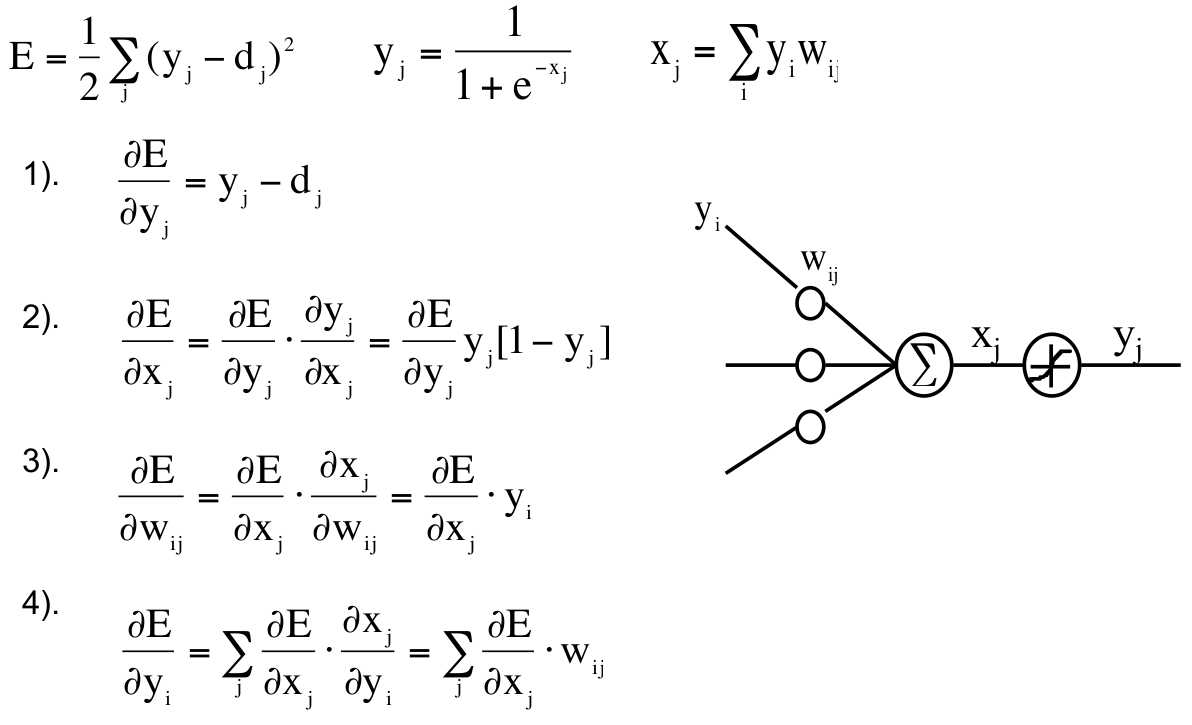
\includegraphics[scale=0.35]{bp}
\end{figure}
The weight update faces different problems: vanishing / exploding gradient, small weights update (slow learning), etc. One way to fix some of the problems is to set a \textit{step size} and \textit{momentum} to the weight update:
\[
\Delta w_{ij}(t) = - \epsilon \frac{\delta E}{\delta w_{ij}(t)} + \alpha \Delta w_{ij}(t - 1) 
\]
$\epsilon$ is the step size (or learning rate) and $\alpha$ is the momentum. The momentum says how much of the last weight update should be added to the current weight update. This will prevent slow training a little.\\[1cm]
Eine weitere Beschleunigung des Trainings erhält man indem für bestimmte Beispiel kein BP angewende wird. Hierbei muss der Fehler groß genug sein, ansonsten wird der Fehler ignoriert.\\[2cm]
Ebenso können wir die Lernrate dynamisch anpassen, um zu verhindern, dass weight updates hin und her springen.
\begin{figure}[h]
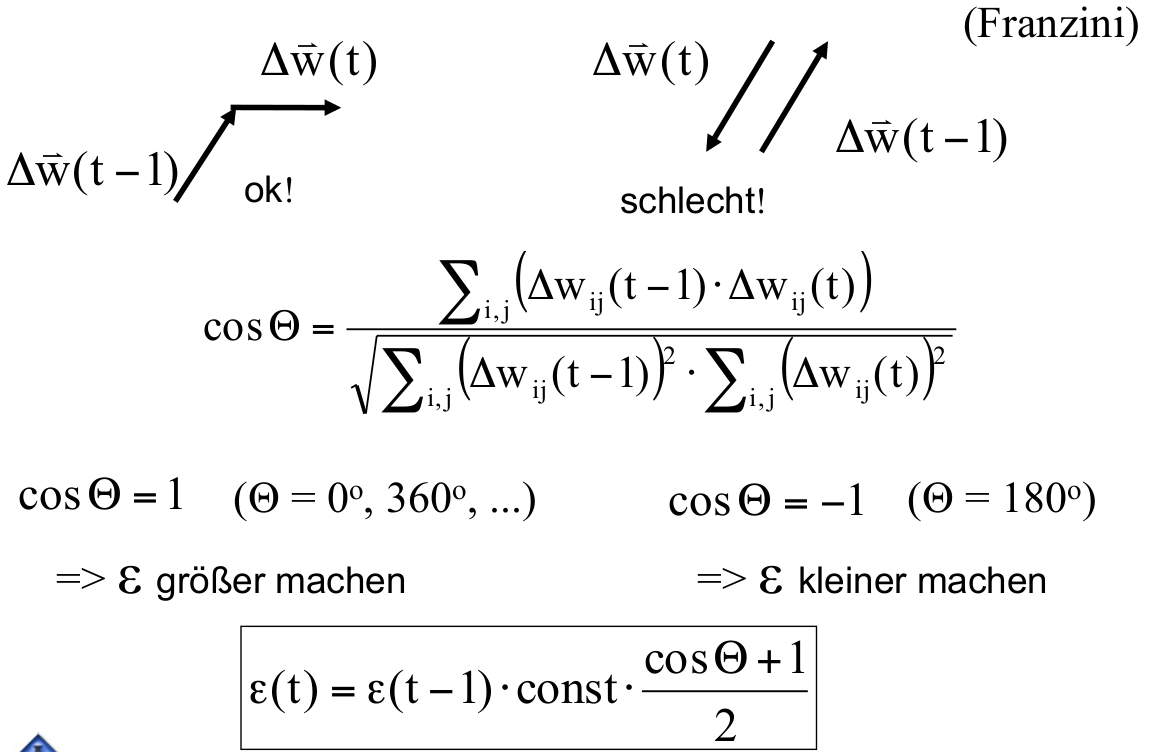
\includegraphics[scale=0.3]{dynamic-learning-rate}
\end{figure}\\[1cm]
Um ein MLP schnell trainieren zu können, kann sich der \textit{Quickprop Algorithmus} eignen:
\[
\Delta w(t) = \frac{s(t)}{s(t - 1) - s(t)} \cdot \Delta w(t-1)
\]
wobei $s(t) = \frac{\delta E}{\delta w_{ij}}(t)$. Jedoch hängt das schnelle Training nicht nur vom Lernalgorithmus ab. The initial weight should be initialist by looking at the activation function and look for the intervall with the biggest derivant.
\textbf{Generalisierung}: The generalization states how well the system will perform on the validation set.\\
Reasons:
\begin{itemize}
	\item Overfitting
	\item too much parameters or too less trainings data
	\item wrong topology
\end{itemize}
Generalization for linear Systems:
\[
\langle \epsilon_{test} \rangle = \langle \epsilon_{train} \rangle + 2 \sigma^2 \frac{p}{n}
\]
Generalization for linear Systems:
\[
\langle \epsilon_{test} \rangle = \langle \epsilon_{train}(\lambda) \rangle + 2 \sigma^2_{eff} \frac{p_{eff}(\lambda)}{n}
\]

Methods to better generalization:
\begin{itemize}
	\item reduce network complexity (weight decay, weight elimination, optimal brain damage, optimal brain surgeon): prevent overfitting
	\item stepwis increase of size of network (cascade correlation, meiosis network, automativ structure optimization): incresae size of network so it can learn
\end{itemize}

\subsection{Regularization}
\label{ssect:regularization}
Regularization is used to prevent overfitting.

\subsubsection{Weight Elimination}
\textit{Weight Elimination} is added to the error to punish the network for large weights ($\lambda$: 0.0001...0.001):
\[
E = MSE + \lambda \sum_{i,j} \frac{w_{i,j}^2}{1 + w_{i,j}^2}
\]
\begin{itemize}
	\item - slow learnin
	\item - worse performance on trainingsdata
	\item + better generalization
\end{itemize}

\subsubsection{Optimal Brain Damage}
\label{sssect:optimal-brain-damage}
Idea: remove certrain connection of the network to reduce the complexity of the network and prevent overfitting. Easy: remove connections with very small $|w_{i,j}|$. Better: remove thos connections which influence the error the smallest (unimportant weights). Therefore calculate:
\[
\frac{\delta E}{\delta w_{ij}^2}
\]
\subsubsection{Cascade Correlation}
\label{sssect:cascade-correlation}
\begin{figure}[h]
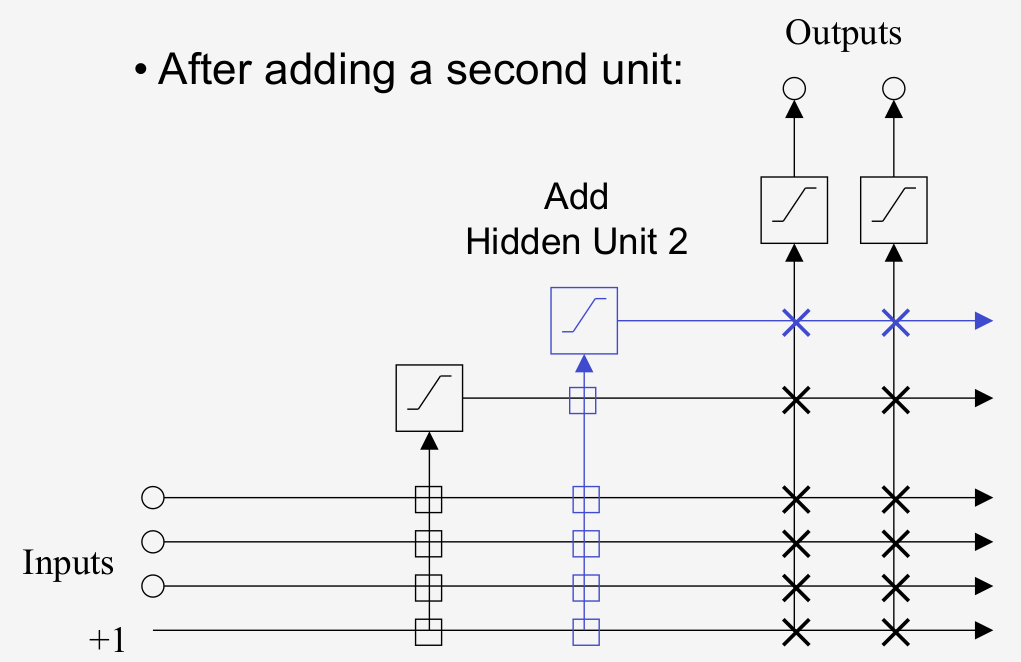
\includegraphics[scale=0.4]{cascade-correlation}
\end{figure}
\begin{itemize}
	\item can create deep networks without a drastic slowdown
	\item amount hidden unis does not need to be estimated empirisch 
	\item each time step only one layer of connections is trained
	\item learns very fast
	\item incremental learning
\end{itemize}

\subsubsection{Meiosis Network}
\label{sssect:meiosis-network}
Idea: adding of hidden unis depends on the ''uncertainty'' of the network. The mean and varianz is learned.
\[
w_{ij}^{*} = \mu(w_{ij}) + \sigma(w_{ij}) \phi(0, 1)
\]
Start with one hidden unit and split unit if
\[
\frac{\sum_i \sigma_{ij}}{\sum_i \mu_{ij}} > 1.0 \: and \: \frac{\sum_k \sigma_{ik}}{\sum_k \mu_{ik}} > 1.0
\]